\documentclass[12pt,letterpaper]{article}
\usepackage{amsmath}
\usepackage{fancyhdr}
\usepackage{graphicx}
\usepackage{alltt}
\usepackage{color}
\usepackage{colortbl}
\usepackage{fullpage}
\usepackage{setspace}
\usepackage{pstricks}
\usepackage{verbatim}
\usepackage{comment}
\usepackage{framed}
\usepackage{listings}
\usepackage{longtable}
\usepackage{pdflscape}
\usepackage{multirow}
\usepackage[config=altsf]{subfig}
\usepackage[utf8]{inputenc}
\usepackage[francais]{babel}
\usepackage[plainpages=false,pdfpagelabels,hypertexnames=false]{hyperref}

%For pdf selection
\usepackage[T1]{fontenc}
\usepackage{lmodern}

%%%%% STYLE %%%%%%%
\topmargin	0in
\topskip	0in
\headheight	0in
\headsep	0in
\parindent	0in
\topsep		0in
\parskip	8pt
\floatsep	0in
%%%%%%%%%%%%%%%%%%%%

%%% SETUP HYPERLINK %%%%%
\hypersetup{
colorlinks 	= true,
linkcolor 	= black}
%%%%%%%%%%%%%%%%%%%%%%%%%

\begin{document}

%%%%%%% COMMANDS %%%%%%%%
\renewcommand{\labelitemi}{$\bullet$}
\newcommand{\unit}[1]{\ \mathrm{#1}}
\newcommand{\degree}{\ensuremath{^\circ}}
%%%%%%%%%%%%%%%%%%%%%%%%%

%%%%%%%%%%%%%%%%%%%%% PAGE TITRE %%%%%%%%%%%%%%%%%%%%%%%%%%%%%%%%%%%%
%%%%%%%%%%%%%%%%%%%%%%%%%%%%%%%%%%%%%%%%%%%%%%%%%%%%%%%%%%%%%%%%%%%%%
\thispagestyle{empty}
\begin{center}
	\vspace{20pt}
	\large{\textsc{
		Intelligence artificielle bio-inspirée\\
	}}
	\vspace{20pt}
	\large{\textsc{
		P02
	}}
	\vfill
	\begin{tabular}{ll}
      Simon Mathieu & 04 450 409 \\
      Steven Denis & 05 667 682 \\
      Michael Janelle-Montcalm & 04 526 123 \\
      Martin Provencher &	05 666 488 \\
	\end{tabular}
	\vfill
	Novembre 2009 \\
	\textbf{Université de Sherbrooke}
	\vspace{20pt}
\end{center}
\clearpage
%%%%%%%%%%%%%%%%%%%%% TABLE DES MATIÈRES %%%%%%%%%%%%%%%%%%%%%%%%%%%%
%%%%%%%%%%%%%%%%%%%%%%%%%%%%%%%%%%%%%%%%%%%%%%%%%%%%%%%%%%%%%%%%%%%%%
\begin{spacing}{0.1}
\tableofcontents
\end{spacing}
\clearpage

\section{Introduction}

\section{Analyse des données} % Steven
% Similitudes entre les canaux (redondance entre 1 et 6, on garde 6)
% Valeurs des maxima et minima sont plus grandes lors d'une chute que lors
% d'une non-chute

\section{Hypothèses simplificatrices}

\subsection{Logique floue}

\subsection{Réseau de neurones} % Mike
% Utilisation seulement des max et min permet d'identifier les chutes
Dans le cas du réseau de neurones, nous avons décidé de détecter s'il y a une chute ou non, peu importe le type de celle-ci. En effet, il s'agit du mandat de base de la problématique. Nous avons utilisé les données découpées telles que fournies dans les échantillons, donc nous nous simplifions la tâche en ne faisant pas de traitement en temps réel. De plus, nous simplifions nos données en entrée en omettant les lectures du capteur 1, étant donné qu'elles sont redondantes avec celles du capteur 6 mais moins significatives. Tel que présenté dans la section d'analyse des données, le maximum et le minimum du signal sont des informations qui semblent suffisantes pour pouvoir détecter l'occurence d'une chute.

\section{Représentation de l'information}

\subsection{Logique floue}

Au niveau de l'algorithme de logique floue, nous avons commencé par éliminer un capteur au complet. Premièrement, ce choix permet de diminuer le coût du système. Deuxièmement, utiliser les trois axes des deux capteurs augmentent de façon drastique le nombre de règles à écrire et alourdi presque inutilement le système. Pour le choix du capteur, nous avons choisit le capteur sous le bras puisqu'en général, il y a de plus grandes variations sur ce capteur.

Pour le traitement des données, nous commençons par réduire l'échantillonnage à 20 Hz afin de diminuer le nombre de valeurs avec lesquels travailler. Par la suite, nous ne gardons que deux valeurs par axe de capteur, le maximum et le minimum de l'échantillon de temps. Ces valeurs sont combinées avec l'équation : $||max|-|min||$ qui permet de déterminer la différence entre les accélérations maximales positives et négatives. Si cette valeur est petite, elle signifie qu'une personne a réussi à appliquer une force équivalente opposée à la chute pour se rattraper ou qu'aucune chute n'a eu lieu. Cette relation a été identifiée après l'analyse des données. Les valeurs caractéristiques de cette équation pour le capteur choisit se retrouvent au tableau \ref{tbl:f_input_val}.

\begin{table}[h]
  \begin{center}
    \begin{tabular} {|c|c|c|c|c|c|c|}
        \hline
        \textbf{Valeurs} & \multicolumn{3}{|c|}{\textbf{Chute}} & \multicolumn{3}{|c|}{\textbf{Non-chute}} \\ \cline{2-7}
         & Axe X & Axe Y & Axe Z & Axe X & Axe Y & Axe Z \\
        \hline
        Minimum & 5.8922  & 0.2753  & 0.4199  & 8.2704  & 1.4687  & 0.2828 \\
        \hline
        Moyenne & 27.3740 & 20.7519 & 22.7897 & 18.1876 & 8.3666  & 11.9716 \\
        \hline
        Maximum & 54.6119 & 61.9975 & 78.1890 & 32.7961 & 17.1413 & 24.1894 \\
        \hline
    \end{tabular}
    \caption{Intervalle de valeurs pour les entrées de l'algorithme de logique floue}
    \label{tbl:f_input_val}
  \end{center}
\end{table}

\subsection{Réseau de neurones} % Steven
% Schéma-bloc du système
% Extraction des caractéristiques (max, min)
% Entrées et sorties (fichiers de données, sorties du script)

\section{Mise en oeuvre}

\subsection{Logique floue}

\begin{figure}
    \centering
    \subfigure[Axe X]{
        \label{fig:f_xi}
        \fbox{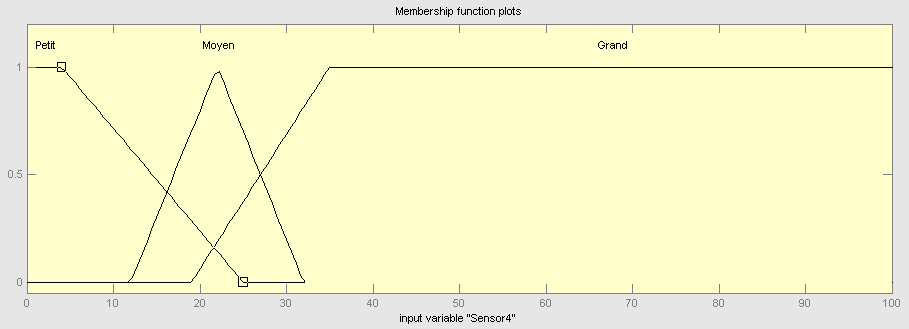
\includegraphics[scale=0.2]{images/f_sensor4.png}}}
    \quad
    \subfigure[Axe Y]{
        \label{fig:f_yi}
        \fbox{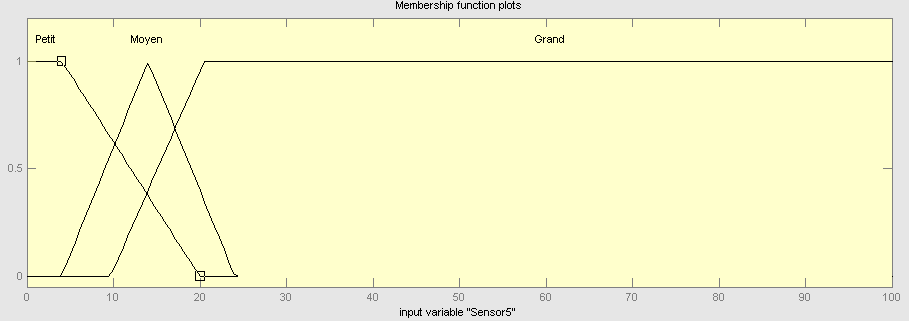
\includegraphics[scale=0.2]{images/f_sensor5.png}}}

    \subfigure[Axe Z]{
        \label{fig:f_zi}
        \fbox{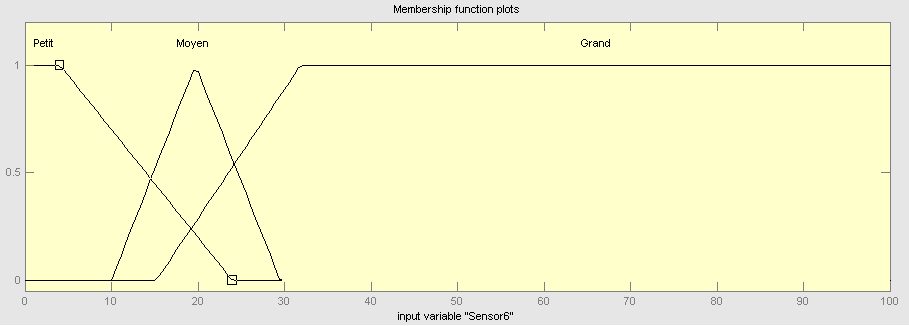
\includegraphics[scale=0.2]{images/f_sensor6.png}}}

    \caption{Équations entrées de l'algorithme de logique floue}
    \label{fig:f_input}
\end{figure}

\begin{figure}
\centering
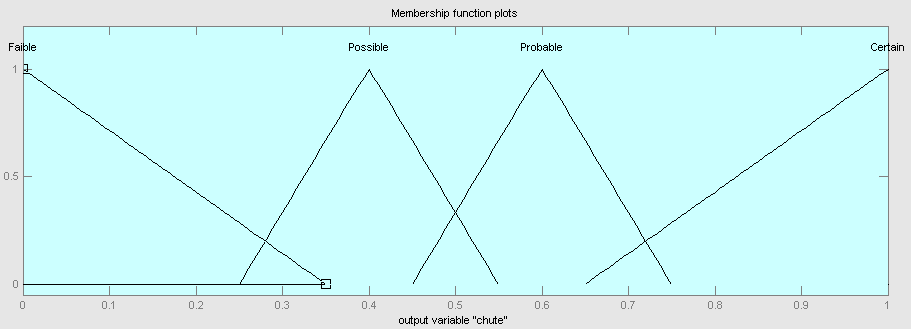
\includegraphics[scale=0.2]{images/f_chute.png}
\caption{Équation de sortie (chute) de l'algorithme de logique floue}
\label{fig:f_output}
\end{figure}

\begin{figure}
    \centering
    \subfigure[Axe X : petit]{
        \label{fig:f_x_petit}
        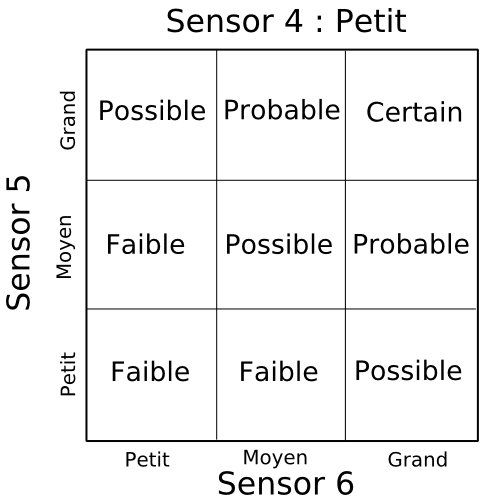
\includegraphics[scale=0.35]{images/f_s4_petit.png}}
    \quad
    \subfigure[Axe X : moyen]{
        \label{fig:f_x_moyen}
        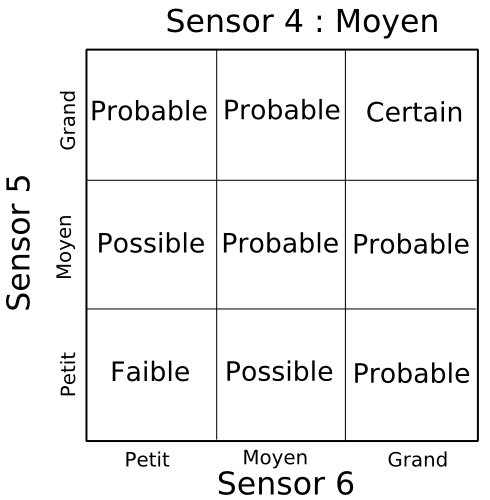
\includegraphics[scale=0.35]{images/f_s4_moyen.png}}
    \quad
    \subfigure[Axe X : grand]{
        \label{fig:f_x_grand}
        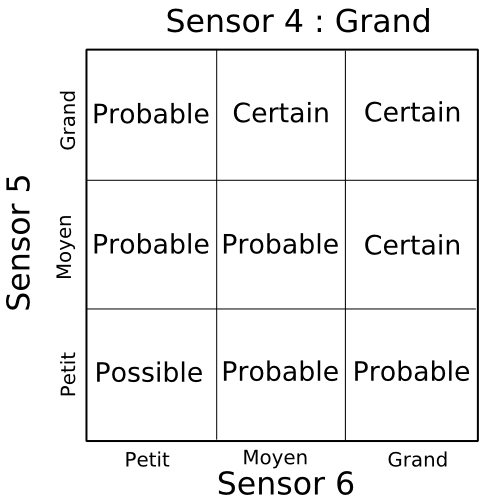
\includegraphics[scale=0.35]{images/f_s4_grand.png}}

    \caption{Règles de l'algorithme de logique floue}
    \label{fig:f_rule}
\end{figure}

% Plus d'explication sur le mélange des valeurs et d'où vient les règles

Pour implémenter cette solution avec un algorithme de logique floue, nous devions passer par quatre étapes. En premier lieu, nous avons déterminé la fuzzification des variables d'entrées. Pour choisir les relations entre les différentes fonction d'appartenance, nous avons utilisé les valeurs disponibles au tableau \ref{tbl:f_input_val}. Notre premier choix a été d'utiliser l'intervalle de 0 à 100 afin de s'assurer de considérer toutes les valeurs d'entrée possible. Puis, nous avons choisi d'utiliser trois fonctions d'appartenance par entrée puisque cela représentait bien notre compréhension et notre expertise du domaine. Les résultats se retrouvent à la figure \ref{fig:f_input}.

En deuxième lieu, nous avons déterminé la défuzzification du système. Puisque nous n'avions pas de contrainte sur les valeurs de sorties, nous avons choisit de garder l'intervalle par défaut, de 0 à 1. Nous avons également choisit d'utiliser 4 fonctions d'appartenance pour faciliter l'écriture des règles et les rendre plus représentative. La relation se retrouve à la figure \ref{fig:f_output}.

En troisième lieu, nous devions définir nos règles pour lier nos entrées fuzzifiées à nos sorties. Selon notre expertise, nous ne voyions pas d'avantage à prioriser un axe plus qu'un autre. Donc, nos règles dépendent du nombre de type d'entrée et non de quel axe la valeur provient. Dans le même ordre d'idée, nous avons choisit de garder le AND pour combiner les entrée et le OR pour combiner les sorties puisque selon notre analyse du domaine, les variables sont indépendantes. Finalement, au niveau de l'aggrégation pour obtenir la valeur finale, nous avons choisit d'utiliser le centroïde puisqu'il s'agit de la valeur par défaut et que nous ne voyions pas l'utilité de la modifier.

% Il faut parler de scaled ou clipped

En quatrième lieu, il faut déterminer le seuil de détection d'une chute et d'une non-chute. Puisque notre sortie varie de 0 à 1, nous avons fait une recherche binaire avec une précision de 2 chiffres après la virgule pour identifier le seuil optimal. Le seuil optimal que nous avons identifier, avec toutes les données fournies, est de 0.42.

\subsection{Réseau de neurones} % Mike
% Données d'entraînement (sujet 5)
% Description de l'évolution du réseau (époques)
% Paramètres d'entraînement (momentum, learning rate)
% Ne converge pas toujours
% – Loi d’apprentissage, nombre d’unités cachées, nombre d’unités de sortie à expérimenter ;
% – Critères d’entraînement et d’évaluation ;
% – Création des ensembles d’entraînement et de test en lien avec l’apprentissage ;
% – Critère de classification et de reconnaissance.

Afin de réaliser notre réseau de neurones, nous avons utilisé les données du sujet 5 comme données d'entraînement et les données du sujet 3 comme données de test. Nous en avons décidé ainsi puisque nous obtenions une meilleure détection avec ces ensembles. De nos échantillons, nous utilisons donc 50\%  de données de test et 50\% de données d'apprentissage.

Pour la réalisation de notre réseau de neurones, nous avons utilisé un algorithme d'entraînement avec rétroprogation de l'erreur. Il s'agit d'un algorithme d'entraînement supervisé qui vise à minimiser l'erreur sur les échantillons d'entraînement. Comme fonction d'erreur, nous avons mis la somme des carrés des différences ($sse$). Par essai et erreur, nous avons trouvé que l'utilisation de 8 unités cachées nous permet de faire converger le système la plupart du temps. Il arrive quand même quelques fois où l'entraînement n'aboutit pas à un système utilisable et nous ne faisons qu'exécuter l'algorithme une nouvelle fois lorsque celà se produit. De manière générale, nous obtenons un graphique d'entraînement qui ressemble à celui présenté à la figure \ref{fig:training_8units}. Nous avons aussi essayé d'utiliser d'autres quantités d'unités cachées, pour voir l'impact de ce paramètre sur le réseau. Nous avons découvert qu'il est possible d'utiliser jusqu'à une vingtaine de neurones. L'augmentation du nombre de neurones amène une convergence plus rapide du système vers les sorties désirées. (Voir les résultats en annexe aux figures \ref{fig:train_1_2}, \ref{fig:train_4_8} et \ref{fig:train_16_24}) L'inconvénient d'augmenter le nombre de neurones est qu'il est plus difficile de faire converger le réseau vers les résultats désirés. Pour 8 neurones, environ un essai sur 10 ne converge pas. Rendu à 24 neurones, il nous a été impossible d'obtenir un réseau utile. Pour détecter une chute, nous regardons si la valeur de la sortie de chute est plus grande que celle de la sortie de non-chute. La reconnaissance s'effectue donc avec la sortie qui a le meilleur score.

\begin{figure}
    \centering
    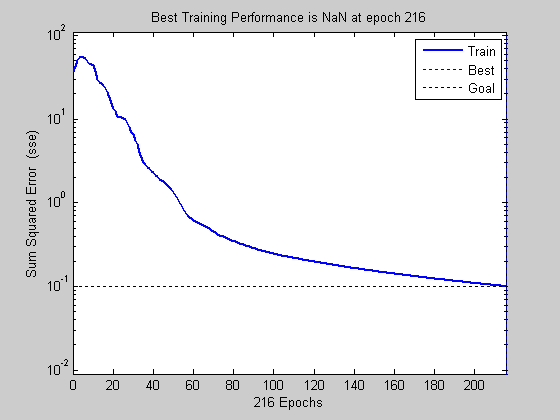
\includegraphics[scale=0.6]{image/training_8units.png}
    \caption{Réduction de l'erreur par entraînement (8 unités cachées)}
    \label{fig:training_8units}
\end{figure}

\subsection{Algorithme génétique}

Originalement, nous voulions utiliser le nombre de piques dans le graphique de la dérivé pour détecter les chutes.
Si le graphique d'un capteur contenait un pique, il s'agit probablement d'une chute. S'il en contient aucun, il
ne s'agît pas d'une chute. S’il en contient plusieurs, il s'agit d'une récupération de chute.

Éventuellement, cette solution fut rejetée en faveur d'une solution offrant de meilleurs résultats, mais nous
présentons tout de même l'implémentation et les conclusions tiré de cette expérience.

Les figures \ref{fig:chute} et \ref{fig:nonchute} montre la différence entre une chute et une récupération de chute.

\begin{figure}[htp]
\centering
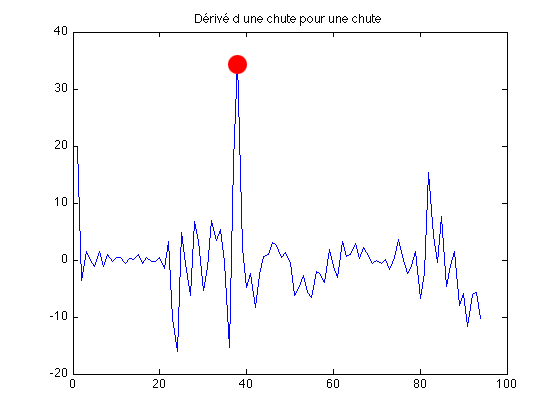
\includegraphics[scale=0.5]{images/piques_chute.png}
\caption{Nombre de piques pour une chute}
\label{fig:chute}
\end{figure}

\begin{figure}[htp]
\centering
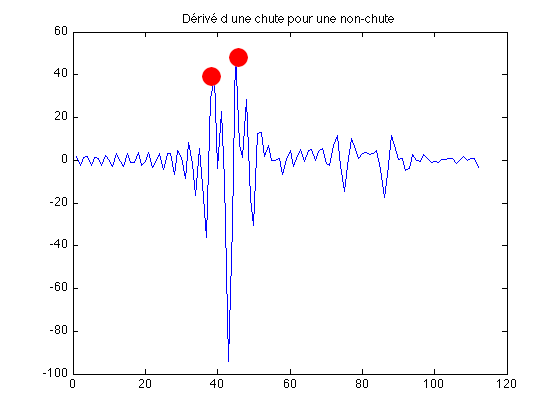
\includegraphics[scale=0.5]{images/piques_nonchute.png}
\caption{Nombre de piques pour une non-chute}
\label{fig:nonchute}
\end{figure}


Pour détecter un pique, nous utilisions une librairie matlab trouvée sur internet. La fonction de détection de pique
possède 4 paramètres permettant de contrôler quels points du graphique sont détectés comme étant des piques.

Comme ces paramètres peuvent prendrent une très grande quantité de valeurs, il s'agissait d'un cas intéressant où utiliser
un algorithme génétique pour trouver des valeurs optimisées. Il est à noter qu'un algorithme génétique ne retourne pas
nécessairement la solution optimale, mais bien une solution possible.

La première étape de la mise en oeuvre fut de manuellement se créer des données d'entrainement. Nous avons donc
observé les graphiques de la dérivé de certains des capteurs et avons estimé le nombre de piques.

Armée de ces données, nous avons ensuite défini une fonction de pertinence qui permet de calculer la distance à laquelle
une donnée est de la valeur réelle.

Nous avons ensuite défini une population d'individu qui se composait d'un ensemble de valeurs représentant les paramètres de la fonction qui trouve les piques.

La prochaine étape consiste a faire reproduire et muter les individus de notre population pour produire la prochaine génération.
Lors de la reproduction et de la mutation, il existe une probabilité que des gènes soient transférés d'un parent à l'enfant et une
probabilité qu'un gène mute. On peut optimiser la vitesse de convergence de l'algorithme en modifiants ces probabilités. Après
expérimentation, nous avons conclu qu'il était mieux de conserver les individus les plus adaptés d'une génération dans la prochaine.
Nous gardons donc les cinq individus les mieux adaptés.

Le choix des individus qui se reproduisent est fait à l'aide d'une fonction aléatoire pondéré de façon à ce que les individus possédant
de meilleurs gènes aient une meilleure probabilité de se reproduire.

Le pseudo-code de notre algorithme est:

\begin{verbatim}
pop = InitPopulation

FOR n generation
  fitnesses = CalculateFitnesses pop
  breeders = SelectBreeders pop
  pop = Reproduce breeders
  pop = Mutate pop

\end{verbatim}


\section{Évaluation des performances}

\subsection{Logique floue}

Tout d'abord, notre algorithme de logique a un taux de détection de 88.5\% : 92\% de reconnaissance de chute et 85\% de reconnaissance de non-chute. Nous considérons cette valeur assez élevée pour considérer cette technique satisfaisante compte tenu de notre compréhension et de notre expertise du domaine limité. En plus, l'algorithme prend, pour s'exécuter, entre 3 et 24 millisecondes avec une moyenne à 9 millisecondes. Donc, nous pourrions facilement implémenter un système de détection de chute à la seconde prêt, en temps réel pour un humain.

En guise de comparaison, nous avons également essayé l'algorithme de logique floue avec seulement les axes Y et Z du capteur 2. Cette implémentation nous donne, à un seuil de 0.40, 83.5\% de détection : 79\% de reconnaissance de chute et 88\% de reconnaissance de non-chute. En temps de calcul, cette solution prend entre 3 et 24 millisecondes avec une moyenne à 9 millisecondes. Donc, puisque les données sont déjà disponibles sans augmentation des coûts en argent ou en temps, il est plus avantageux d'utiliser le système avec les 3 axes.

\subsection{Réseau de neurones} % Mike
% Taux d'identification (avec explications des variations selon les paramètres)
% Performance avec les données d'entraînement, puis les données de test
% Différence des résultats selon le nombre d'unités cachées

La performance de notre algorithme avec les données d'apprentissage est parfaite. Ceci est dû au fait que nous fixons un seuil global d'erreur sur les données de test d'une valeur de 0.1. L'entraînement de notre réseau se termine lorsque la somme des carrés des erreurs de chaque sortie est sous ce seuil pour l'ensemble des données d'apprentissage, ce qui assure que toutes les données d'apprentissage sont bien identifiées.

Les réseaux de neurones que nous générons obtiennent habituellement de bons taux de détection avec les données de test. Le tableau \ref{tbl:neural_results} montre les taux de réussite, en faisant varier la taille de la couche cachée. Nous observons qu'en général, augmenter le nombre de neurones amène une meilleure détection. Le meilleur réseau que nous avons observé possédait 16 neurones et affichait un taux de reconnaissance de 96\%. Nous n'avons cependant pas opté pour celui-ci puisqu'il a fallu plusieurs essais avec notre système avant de le générer. Aussi, le réseau avec 1 seul neurone a requis plusieurs essais avant de converger. Évidemment, lorsque nous analysons la structure, il apparaît qu'en ayant moins d'unités dans la couche cachée que dans la couche de sortie, nous diminuons les chances de distinguer les sorties. Il est même surprenant que nous ayons pu générer un réseau valide avec cette configuration. Donc, après avoir analysé l'impact du nombre d'unités cachées, nous avons fixé notre forme à 8 neurones.
\begin{table}
\centering
\begin{tabular}{|c|c|c|c|}
    \hline
    Nombre de neurones & Reconnaissance chutes & Reconnaissance non-chutes & \% reconnaissance \\ \hline
    1 & 57\% & 100\% & 74\%  \\ \hline
    2 & 96\%  & 88\% & 93\% \\ \hline
    4 & 96\% & 88\% & 93\% \\ \hline
    8 & 93\% & 98\% & 95\% \\ \hline
    16 & 94\% & 98\% & 96\% \\ \hline
\end{tabular}
\caption{Résultats obtenus sur les données de test pour le réseau de neurone}
\label{tbl:neural_results}
\end{table}

L'autre paramètre que nous avons étudié est la quantité et la diversité des données d'apprentissage. Nous avons fait les tests précédents en utilisant les données du sujet 5 comme base pour l'apprentissage. Dans ce test, nous remarquons une meilleure détection en utilisant le sujet 5.

\begin{table}
\centering
\begin{tabular}{|c|c|c|c|}
    \hline
    Apprentissage & Reconnaissance chutes & Reconnaissance non-chutes & \% reconnaissance \\ \hline
    Sujet 3 &  &  &   \\ \hline
    Sujet 5 & 93\%  & 98\% & 95\% \\ \hline
    Sujet 5 + 40\% Sujet 3 &  &  &  \\ \hline
    60\% Sujet 5 + 60\% Sujet 3 & & & \\ \hline
\end{tabular}
\caption{Résultats obtenus en variant les données d'apprentissage, pour 8 unités cachées}
\label{tbl:neural_results_2}
\end{table}
\subsection{Algorithme génétique}

Dans notre cas, l'algorithme générique nous a permis de converger plutôt rapidement vers une solution suffisamment optimale.

Malheureusement, trouver le nombre de piques dans une fonction n'est pas un problème simple. La librairie que nous utilisions
s'est avérée insuffisante pour détecter les pics correctement dans les données que nous avions.

Nous avons manuellement ajusté les paramètres de l'algorithme génétique, tel que la probabilité de mutation et le nombre de génération. 
La validité des résultats étaient vérifier à l'aide de la fonction de la fonction de pertinence. Plus la fonction de pertinence retourne
une haute valeure, plus l'individu est aptes a survivre. 

\begin{table}[h]
  \begin{center}
    \begin{tabular} {|l|l|}
        \hline
        Nombre de génération & 60 \\
        \hline
        Nombre de chromosones & 250 \\
        \hline
        Probabilité de crossover & 0.8 \\
        \hline
        Probabilité de mutation & 0.02 \\
        \hline
    \end{tabular}
    \caption{Paramètres de l'algorithme génétique}
  \end{center}
\end{table}

Nous avons aussi modifié la fonction de pertinence pour quel attribut une plus grande valeur aux graphiques ayant plus qu’un pic.
Nous avons dû faire cette optimisation, car trop de graphiques avaient un seul sommet, ce qui permettait a notre algorithme d'avoir une bonne
performance en identifiant 1 sommet pour tous les graphiques.

Les résultats obtenus sont affichés dans la table \ref{tab:genparam}.

\begin{table}[h]
  \begin{center}
    \begin{tabular} {|l|l|}
        \hline
        \bf{Paramètre} & \bf{Valeur} \\
        \hline
        SlopeThreshold & 2.1067 \\
        \hline
        AmpThreshold & 3.2950 \\
        \hline
        SmoothWidth & 1.2083 \\
        \hline
        PeakGroup & 24.1062 \\
        \hline
    \end{tabular}
    \caption{Paramètres trouvés à l'aide de l'algorithme génétique}
    \label{tab:genparam}
  \end{center}
\end{table}

Avec ces données, nous obtenons une pertinence de 62.3438 où une détection correcte d'un pique vaut 75 sinon elle vaut 100 divisé par l'erreur.
Au niveau du temps d'exécution, l'exécution d'une fonction génétique nécessite beaucoup de ressources. Par contre, il est à noter que
cette quantité de travail est bien moindre que celle nécessaire avec un algorithme plus conventionnel. Aussi, pour notre application, nous n'avons
qu'a rouler une fois l'algorithme pour obtenir les paramètres optimisés. Une fois ces paramètres obtenus, nous pouvons les réutiliser à chaque exécution.

\section{Observations et perspectives futures}

\pagebreak
\section{Annexe}

\subsection{Variation du nombre d'unités cachées}
Voici les résultats de l'entraînement pour les différents nombres d'unités cachées. Le graphique représente la somme des carrés des différences entre le résultat obtenu et la sortie attendue.
\begin{figure}
    \centering
    \subfloat[Entraînement avec 1 neurone]{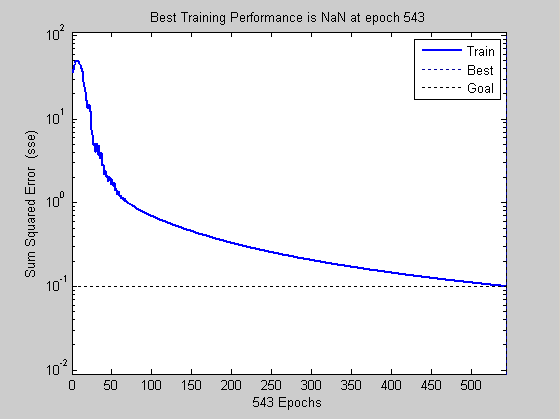
\includegraphics[scale=0.40]{image/training_1units.png} \label{fig:training_1units}}
    \hspace*{0.5in}
    \subfloat[Entraînement avec 2 neurones]{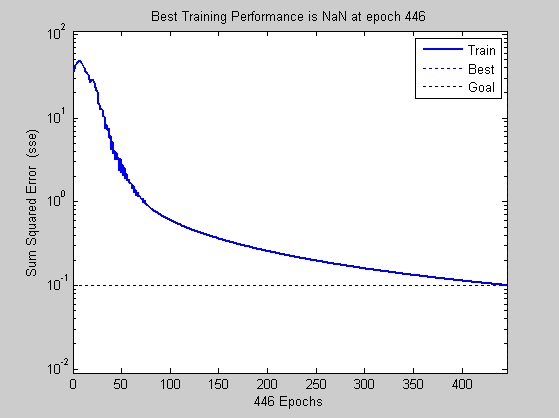
\includegraphics[scale=0.40]{image/training_2units.png} \label{fig:training_2units}}
    \caption{Entraînement avec 1 et 2 neurones}
    \label{fig:train_1_2}
\end{figure}

\begin{figure}
    \centering
    \subfloat[Entraînement avec 4 neurones]{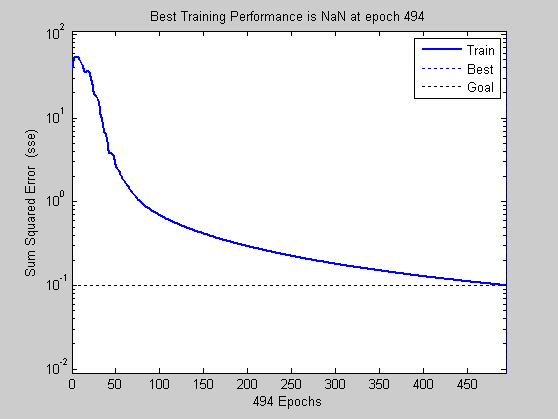
\includegraphics[scale=0.40]{image/training_4units.png} \label{fig:training_4units}}
    \hspace*{0.5in}
    \subfloat[Entraînement avec 8 neurones]{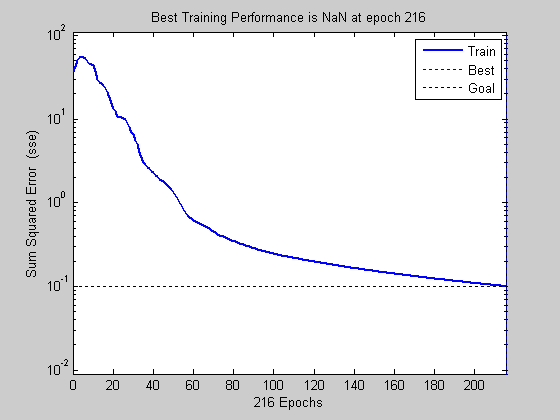
\includegraphics[scale=0.40]{image/training_8units.png} \label{fig:training_8units_annex}}
    \caption{Entraînement avec 4 et 8 neurones}
    \label{fig:train_4_8}
\end{figure}

\begin{figure}
    \centering
    \subfloat[Entraînement avec 16 neurones]{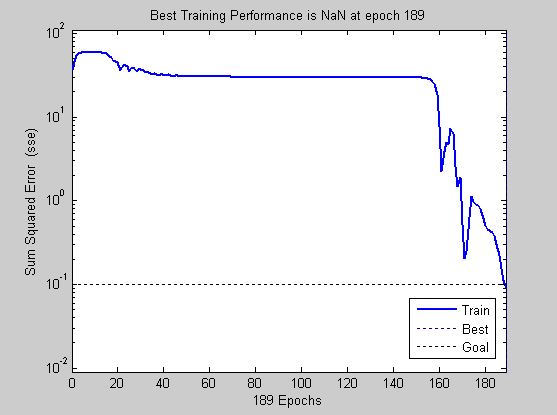
\includegraphics[scale=0.40]{image/training_16units.png} \label{fig:training_16units}}
    \hspace*{0.5in}
    \subfloat[Entraînement avec 24 neurones]{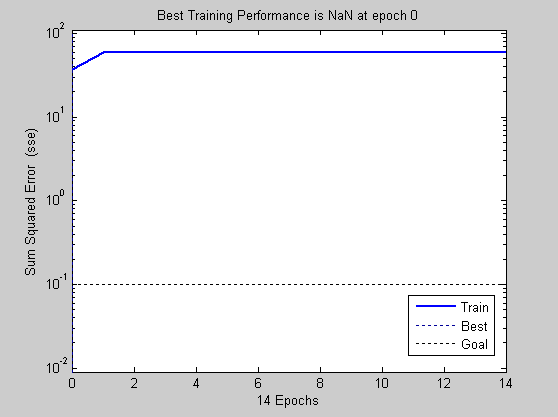
\includegraphics[scale=0.40]{image/training_24units.png} \label{fig:training_24units}}
    \caption{Entraînement avec 16 et 24 neurones}
    \label{fig:train_16_24}
\end{figure}

\end{document}
